\section{Introduction}

\begin{frame}
	\frametitle{Reinforcement Learning}
	
	\begin{center}
		\begin{tikzpicture}
			\node at (0,0) [draw=white,ultra thick,inner sep=0pt]
			{
				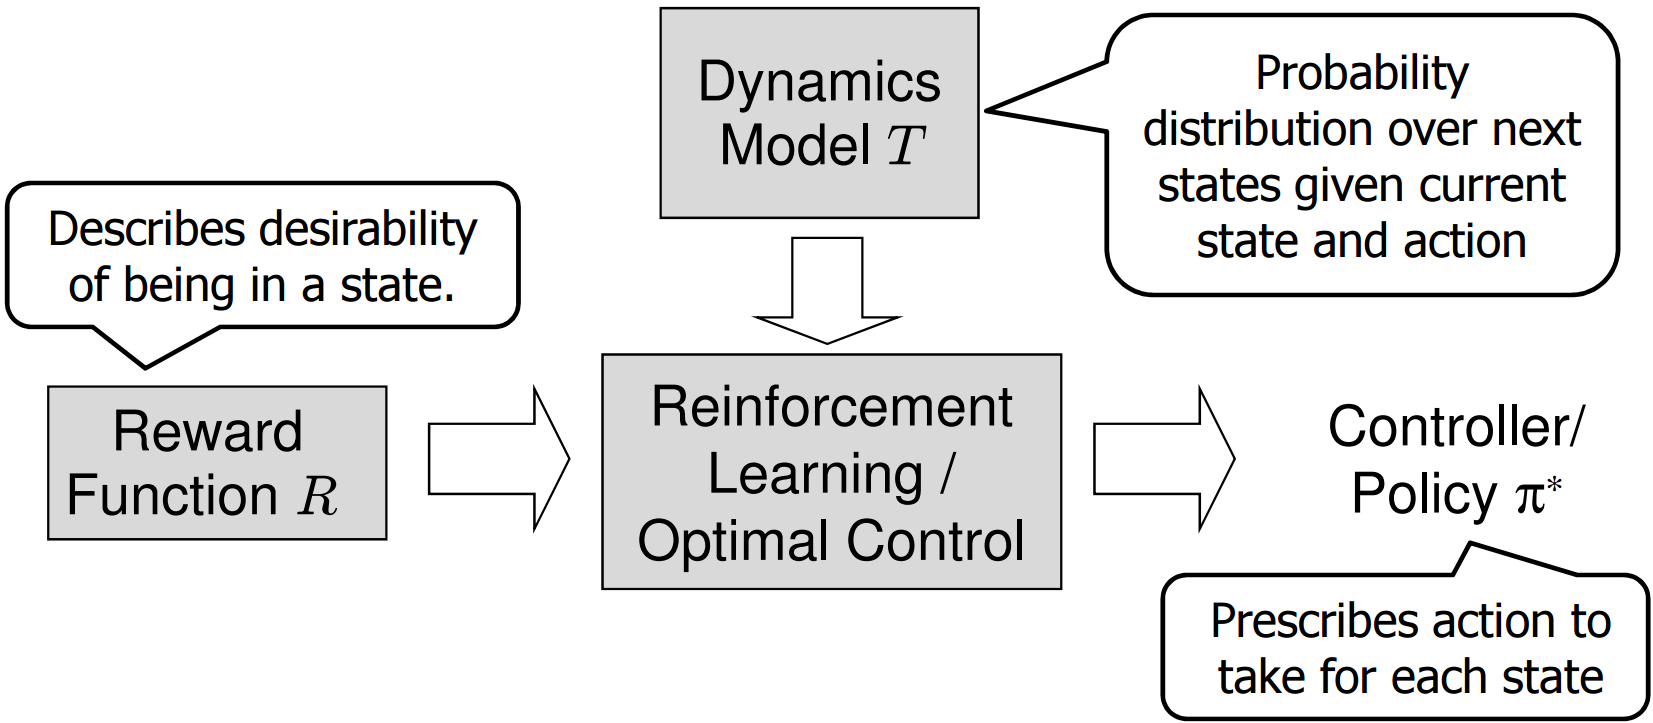
\includegraphics[scale=0.2]{Figures/RL.png}
			};
		\end{tikzpicture}
	\end{center}
	
	\vspace{-0.5cm}
	
	\textcolor{red}{Inverse RL:} \\
	\hspace{1cm}\textcolor{red}{Given $ \pi^* $ and $ T $, can we recover $ R $?\\
	\hspace{1cm}More generally, given execution traces, can we recover $ R $?}
\end{frame}

\begin{frame}
	\frametitle{Motivation for Inverse RL}
	
	\Large
	
	\vspace{0.3cm}
	
	\begin{itemize}
		\item \textbf{Scientific inquiry}
			  \begin{itemize}
				  \item Model animal and human behavior (\emph{Russell et al.}, 2000)
				  \vspace{0.15cm}
				  \item Activity forecasting (\emph{Ziebart et al.}, 2012)
			  \end{itemize}
		\vspace{0.2cm}
		\item \textbf{Imitation learning}
			  \begin{itemize}
				  \item Presupposition: reward function provides the most succinct and
				  		transferable definition of the task
				  \vspace{0.15cm}
				  \item has enabled advancing the state-of-the-art in various robotic domains
			  \end{itemize}
		\vspace{0.2cm}
		\item \textbf{Agent modeling (adversarial and cooperative)}
		\vspace{0.2cm}
		\item ...
	\end{itemize}
\end{frame}
